% Figure: 2D alpha x n_eff joint ablation heatmap

\begin{figure}[h]
\centering
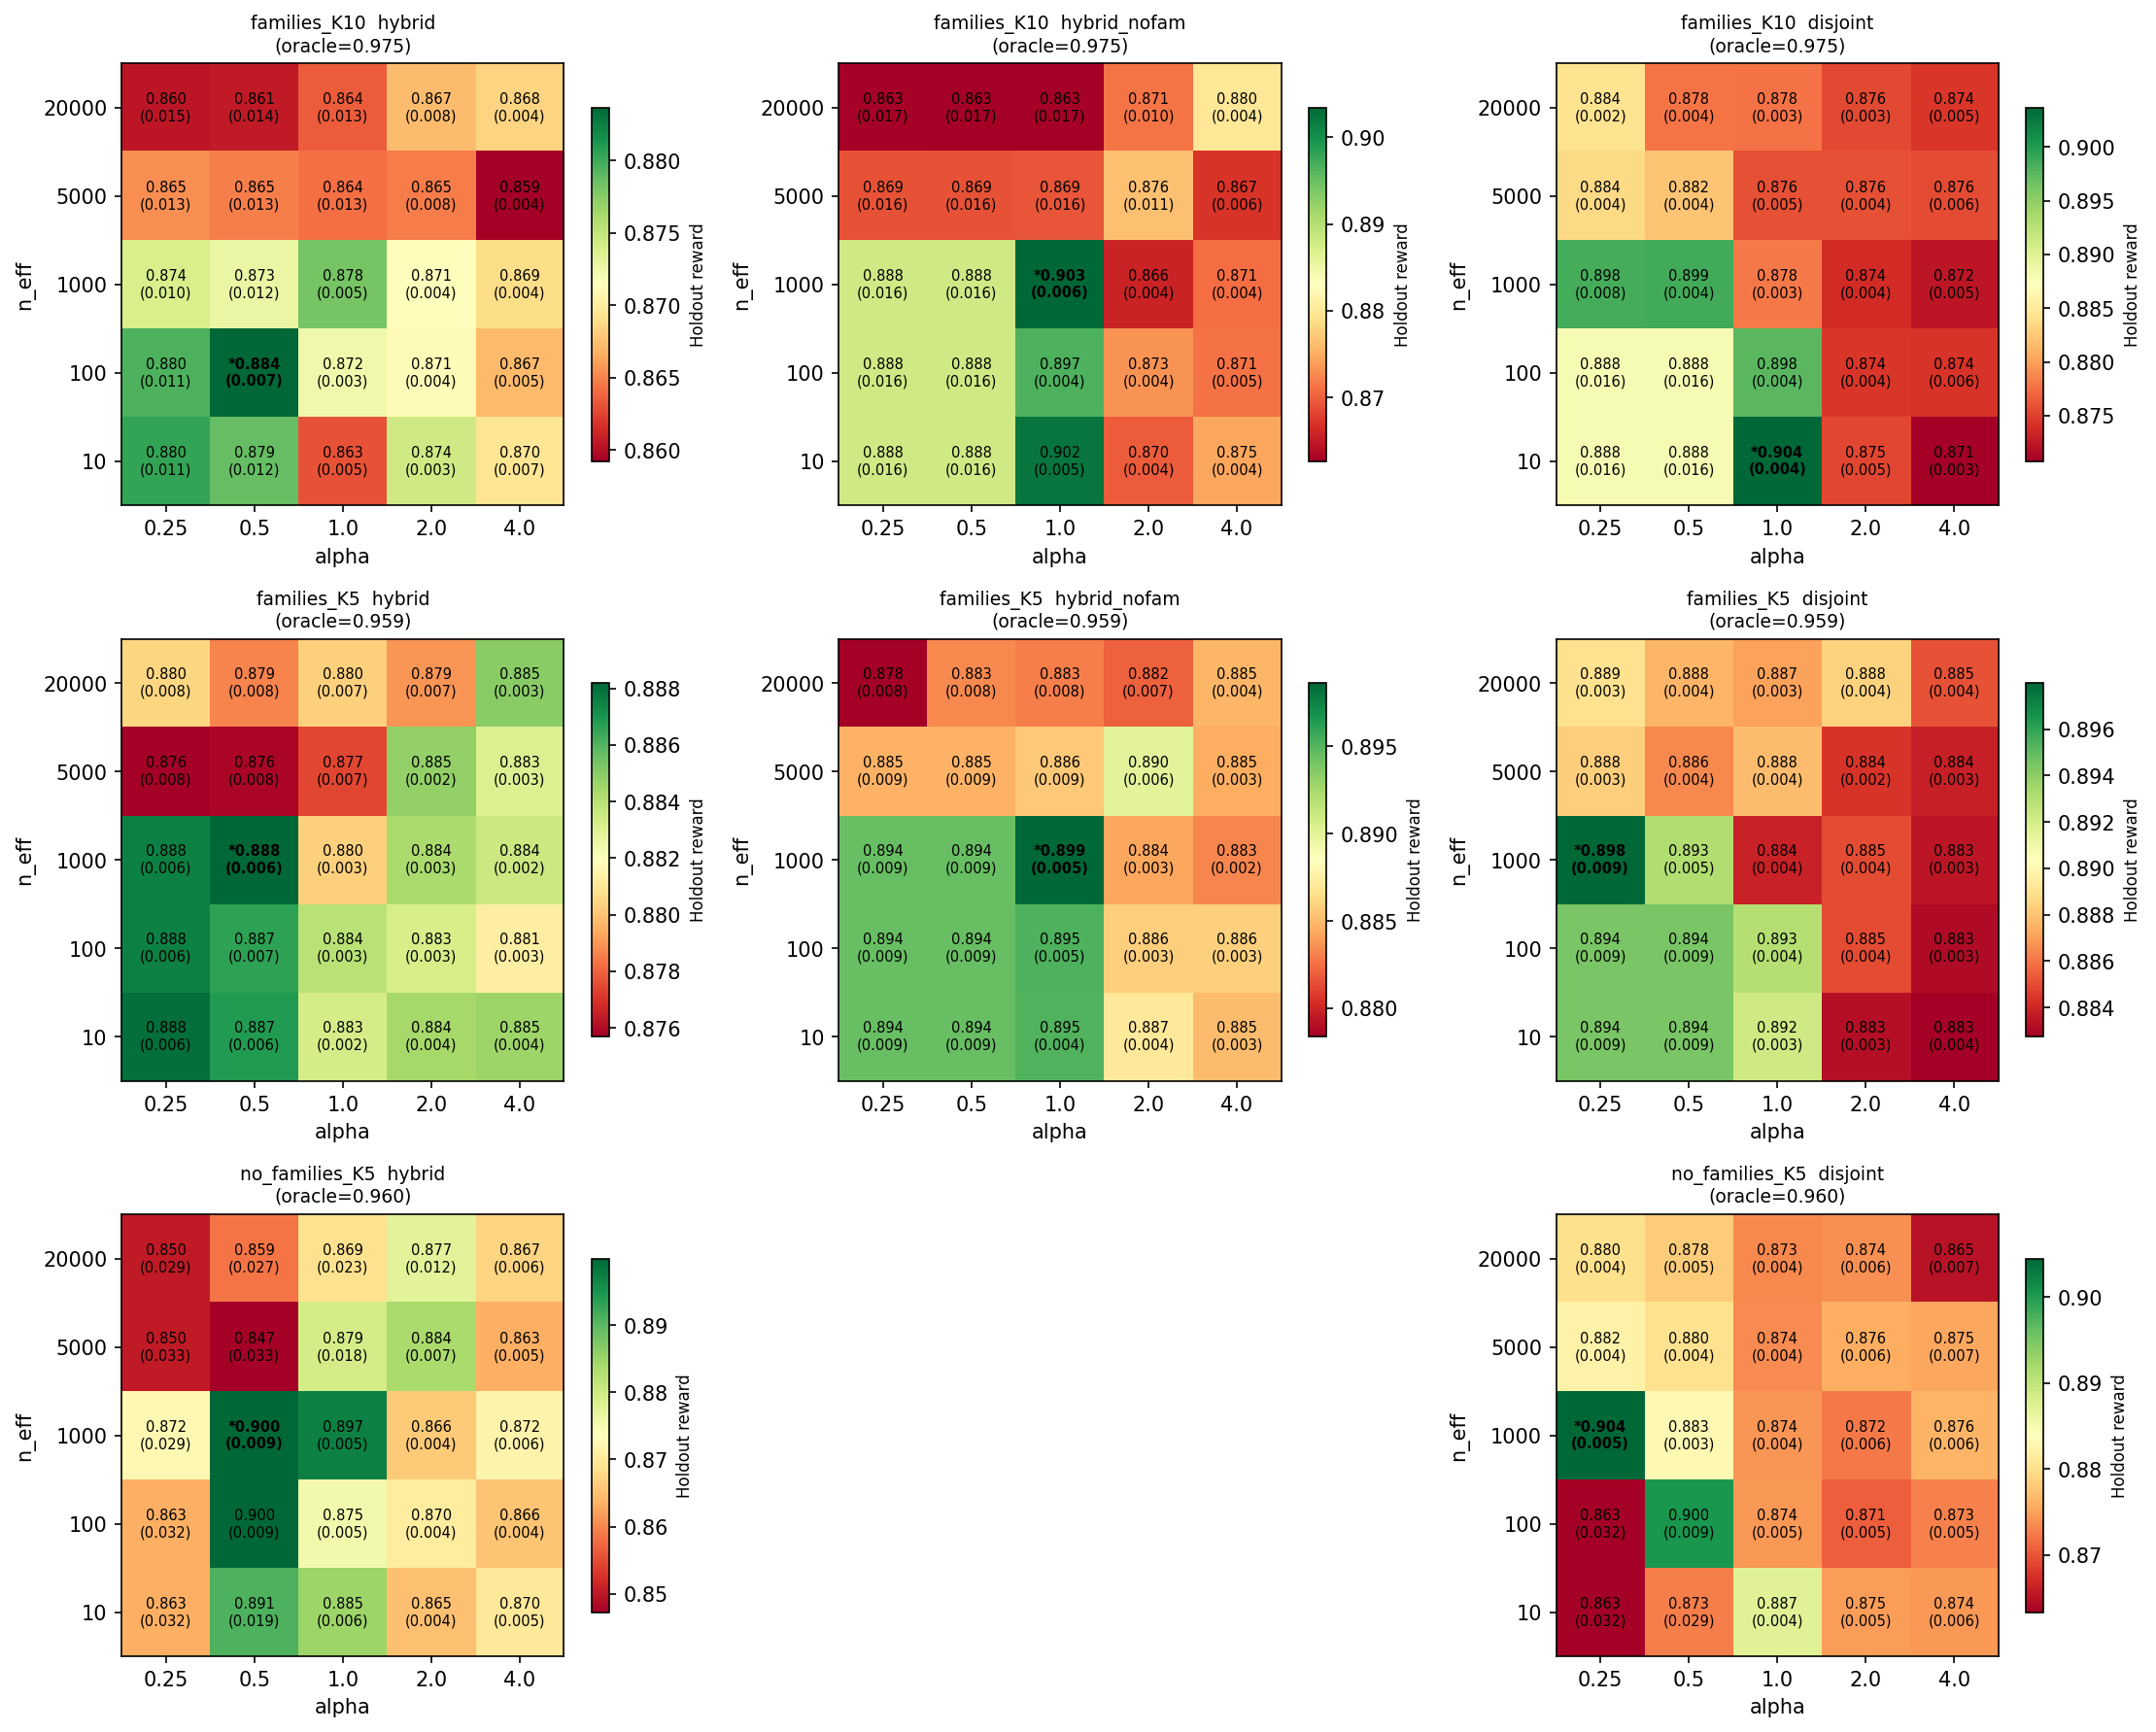
\includegraphics[width=\textwidth]{H_alpha_neff_ablation/results/alpha_neff_grid_figure.png}
\caption{%
    \textbf{Joint $\alpha \times \neff$ ablation} (2$\times$2 heatmap:
    rows = $K$, columns = policy).
    Each cell shows holdout reward (mean $\pm$ 95\% CI, 20 seeds).
    Starred (*) cells mark the per-panel optimum.
    The global optimum ($\alpha{=}0.25$, $\neff{=}1{,}000$, Disjoint)
    achieves $0.907$ at $K{=}5$ and $0.904$ at $K{=}10$, outperforming
    the default ($\alpha{=}0.5$, $\neff{=}10$) by ${\sim}3$\,pp.
    At low $\alpha$, the reward landscape is sharply peaked around
    $\neff{=}1{,}000$; at $\alpha \geq 1.0$, $\neff$ has negligible
    effect, confirming an $\alpha$--$\neff$ interaction.
}
\label{fig:alpha_neff_grid}
\end{figure}
